\documentclass[a4paper]{article}


\usepackage[english]{babel}
\usepackage[utf8]{inputenc}
\usepackage{graphicx}
\usepackage{amsmath}

\begin{document}
 
Let's consider a graph that have only two vertices and any number of edges. All the relaxed edges will lead from the starting vertex to the other one. Also the edge will be relaxed if and only if it's weight less then weights of all previously considered. Our implementation of Dijkstra algorithm pass through the edges that start in particular vertex in order they were given to the algorithm. So if we consider the list of edges in order they are given to the algorithm the relaxed edges in it will be in descending order by weight as in the figure below.

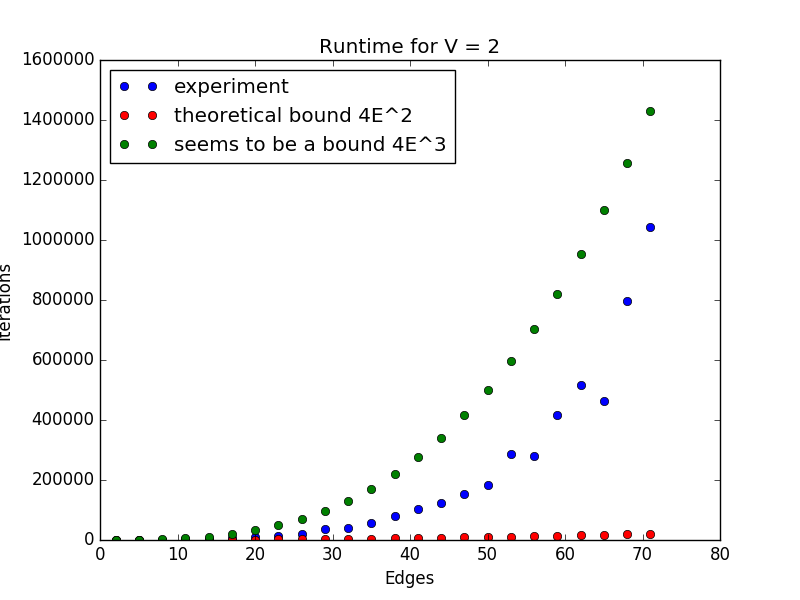
\includegraphics{pic/dense_graph.png}

Despite relaxed edges let there be two additional edges at the beginning of the list with the weight $1.0$ and at the end with weight $0.0$. They are only needed for the following definitions of $d_i$ and $\delta_i$. Let $d_i$ be the number of unrelaxed edges in the interval between $i$-th and $(i + 1)$-th relaxed edges. Also let $delta_i$ be the difference of weights of these edges.

Now we can introduce the potentional function:
$$\Phi = \sum_i d_i \delta_i$$
To use multiplicative drift-theorem we need to finde the expecation of the expected difference of potential function afte one iteration of algorithm. It will be sum for every unrelaxed edge it't probability t be chosen multiplicated by the probability to orient it from the starting vertex to the other one and by the difference in the potential function caused by replacing this edge. The last factor can be bounded from the top by $\delta_i$ (if the unrelaxed edge is in the $i$-th interval).
$$E(\Phi_t - \Phi_{t + 1} | \Phi_t) \ge \sum_{\text{unrelaxed edges}} \frac{1}{E} \frac{1}{4} \delta_i = \frac{1}{4E} \sum \delta_i = \frac{1}{4E} \Phi_t$$

By the multiplicative drift-theorem we have:
$$T \le 4E \left(1 + \ln\frac{\Phi_0}{\Phi_{min}}\right)$$
$Phi_0$ is $E$ but $\Phi_{min}$ can be as small as possible. But if we take any sequense $\{\eps_i\}_{i = 1}^{+\infty}$, that tends to zero, we can bound runtime in the following way:
$$T \le p(\Phi_{min} > \eps_1)T(\eps_1) + \sum_{k = 2}^{+\infty}p(\eps_{k-1} \ge \Phi_{min} > \eps_k)T(\eps_k)$$
where $T(\eps_k) = 4E \left(1 + \ln{E/\eps_k)\right)$.

Because of independence of evens $p(\eps_{k-1} \ge \Phi_{min} > \eps_k) = p(\eps_{k-1} \ge \Phi_{min})p(\Phi_{min} > \eps_{k-1})$. The event when $\Phi_{min} > \eps_k$ takes place when every edge becoming relaxed has weight not closer then $\eps_k$ to the weights of all previously relaxed edges. If we call ``the ristricted area'' all the possible weights from $[0.0; 1.0]$ that are closer then to previosly relaxed edges after $i$ of them were relaxed, then the probability of putting new edge to the non-restricted area is $(1 - 2i\eps_k)$ because every every adds $2\eps_k$ to the restricted area when relaxed.

 
\end{document}
